%%%%%%%%%%%%%%%%%%%%%%%%%%%%%%%%%%%%%%%%%%%%%%%%%%%%%%%%%%%%%%%%%%%%%%%%%%%%%%%%%%%%%%%%%%%%%%%%%%%%%%
%
%   Filename    : chapter_2.tex 
%
%   Description : This file will contain your Review of Related Literature.
%                 
%%%%%%%%%%%%%%%%%%%%%%%%%%%%%%%%%%%%%%%%%%%%%%%%%%%%%%%%%%%%%%%%%%%%%%%%%%%%%%%%%%%%%%%%%%%%%%%%%%%%%%


\chapter{Review of Related Literature}
\label{sec:relatedlit}

This section surveys two types of traffic models: (a) those that do not consider weather data, and (b) those that do consider weather data. For each traffic model, we compare the data used, their research methodology, the modeling approach, and their evaluation strategy. 



\section{Materials}

\subsection{Traffic Data}
% traffic data
The surveyed traffic models used different types of traffic data for training their models. The modified Biham-Middleton-Levine (M-BML) model used real-time traffic density and evolution rules as its input \shortcite{M-BML:2016}. On the other hand, an artificial neural network (ANN) model used real-time traffic volume per 5-minute interval as its input \shortcite{ANN:2016}. Aside from the ANN model, an H-ARIMA model also used traffic volume together with speed data \shortcite{pan2012utilizing}. These data were collected from 800 loop detectors different stationed at different highways in Los Angeles, California.

On the other hand, the knowledge-based model used vehicle GPS data and intersection delay \shortcite{Lee:KnowledgeBase}. This model used location-based services such as GPS to collect data in real time. The data collected were the position of the vehicle (cartesian coordinates), traveling speed, direction, and status (idle or not). In addition, intersection delay, the average time it takes for a vehicle to make its turn in intersections, was also taken into account as an input for this model.

The Deep Belief Network (DBN) with Data Fusion model, the rainfall integrated Recurrent Neural Network the Stationary Wavelet Transform - Autocorrelation Neural Networks (SWT-ACNN) model also collected traffic volume \shortcite{koesdwiady:2016, dunne:2013}. In the DBN with Data Fusion model, traffic volume is measured every 15 minutes for four months to generate a 15-minute traffic prediction. In the SWT-ACNN model, traffic volume is measured hourly in 14 days to generate a 1-hour traffic prediction. The RNN using LSTM was initially collected in 2-minute traffic volume for 2 months \shortcite{Jia:2017}. Traffic data was resampled from 2 minutes and 30 minutes to generate 10 and 30-minute prediction. The DBN with Data Fusion and LSTM in RNN collected traffic data from freeways in USA and China, respectively. The SWT + ACNN collected traffic data from city roads in Ireland. Meanwhile, the MLRA model collected traffic volume together with traffic speed and travel time in road segments in surrounding Ocean Beach in Seoul, South Korea from July and August 2013 \shortcite{Lee2015}. 

\subsection{Weather Data}
% weather data
The weather data used in weather-aware models also differ from one to the other depending on the presence of these variables in their data, and the correlation between weather and traffic. The DBN with Data Fusion collected weather data from 16 different weather stations for 4 months \shortcite{koesdwiady:2016}. The weather data includes information for different weather variables such as weather condition, temperature, humidity, wind gust and speed, visibility, dew point, and cloud layer height. After correlating weather variables with traffic condition, the DBN with Data Fusion model made use of temperature, wind gust, and weather condition as their final weather input data.

RNN that uses LSTM used historical hourly rainfall intensity data \shortcite{Jia:2017}. The study's weather data was resampled to fit the traffic data sampled from 2 to 30 minutes. 

In training the SWT-ACNN model, historical weather data is collected from one weather station \shortcite{dunne:2013}. The weather data consisted of hourly rainfall record of rainfall level measured in millimeters per hour during the weekdays in 14 days. However, in the actual run time of the model, current weather condition is collected real-time.

In training the MLRA model, 48 individual weather variables were analyzed through regression. In addition, dummy variables, such as the days of the week, were used. Because there are too many highly-correlated independent variables, regression analysis was used to remove these, avoiding redundancy. Their final input for weather variables is temperature, humidity, and rainfall. 




\section{Research Methodology}
% M-BML
The procedure of predicting traffic of the M-BML model can be summarized in three steps \shortcite{M-BML:2016}. First, traffic data input is initialized. Based on the traffic density of each road segment in the route, they obtained the average traffic density of each route. Then, the number of vehicles in the M-BML model is initially distributed based on the traffic density of each route.

Second, the M-BML model runs the system. After the model is initialized, a set of evolution rules on how the M-BML model runs is defined: (1) If the next cell is empty, only the vehicles heading \textit{east} can move through one cell at an odd step time; and if the next cell is empty, only the vehicles heading \textit{north} can move through one cell at an even step; and (2) to conserve the number of vehicles in each line, the boundary conditions are periodic. After defining all evolution rules, the system sets a threshold to confirm the jammed area and gradually decreases it to confirm the jammed cells.

Third, different mapping strategies are used to plot the coordinates of the jammed cell in the M-BML model to the intersections in the real-life traffic network. When the model stops running, then the jam value of each cell is confirmed. 

% Knowledge-based
Meanwhile, the knowledge-based model undergo four phases as part of its prediction process. The first phase involves the generation of traffic information. This involves the collection and transformation of mined data. This is collected through reports sent to the onboard unit (OBU) of the location-based service application. The mined data will be used to generate real-time traffic information, which is stored and be used as part of the model's real-time predictor's inference.

The next phase involves the mining of the traffic patterns. Using the data from the first phase, traffic patterns will be derived from the historical database. The traffic information generation module will then aggregate these data from the same vehicle and classify them based from four traffic patterns: right-turn delay (RTD), left-turn delay (LTD), spatial and temporal aggregation (STA), and through delay (TD). These processed data will be stored into a journey set table for the model's historical predictor's inference.

After the raw data have been preprocessed and patterns have been mined, an inference engine for the model is developed. This phase will involve the rule construction of the model. These will be based on traffic patterns and meta-rules defined by domain experts. Rules derived from the historical journey set are converted to an if-else ruleset. Meanwhile, meta-rules defined by domain experts include real-time external traffic events such as road accidents. 

Lastly, an expert system is developed to make use of these generated and preprocessed traffic information. Three inputs are used in the expert system: an origin-destination pair, start time, and external event module. These are used together with the historical and real-time predictor for the knowledge-based model.

% ANN
\shortciteA{ANN:2016}, on the other hand, have developed a model using ANN approach. For their training, four inputs were taken and the output was predicted. Then, together with the input from the input layer, this predicted output is stored in the context layer which is fed in next iteration for predicting the next one. The process of prediction consists of two subprocesses: feed-forward and backpropagation. During backpropagation, the weights are adjusted depending upon the error.

% H-ARIMA
In the H-ARIMA model, \shortciteA{pan2012utilizing} used traffic parameters like traffic volume and speed to analyze an auto-regression algorithm called Auto-Regressive Integrated Moving Average (ARIMA) and a model that uses average historical data called Historical Average Model (HAM). They were able to infer that because ARIMA uses real-time data, it is only optimal for short-term future prediction while HAM is better to use when doing long-term prediction because it uses the average historical data of a given day of week and time of day. Trying to utilize both models’ advantages, they developed a hybrid model that distinguishes whether it is more suitable to use ARIMA or HAM given a situation. In training the model, it first initializes the dataset of all historical data on a given day at a given time. This dataset is then used to test both models to determine their prediction error. From there, the model can determine which submodel to use.

% SWT-ACNN
In  \shortciteA{dunne:2013}, the SWT-ACNN model decomposes input data, either traffic or weather or both, using Stationary Wavelet Transform (SWT) into approximations, and feeds these into the ANN, and generates an output which is recombined using Inverse SWT (ISWT). This generated and recombined output is the predicted traffic flow. Before feeding the decomposed data into the neural network, the decomposed data is auto-correlated to determine the correlation between observations at different lags and to determine the most influential point of the approximations. Additionally, the coefficients for both the weather data and traffic flow are used as input to the neural network at each level of decomposition.

The model framework of the SWT-ACNN is comprised of two parts, the Dry Model and the Wet Model \shortciteA{dunne:2013}. The model first determines whether is it currently raining. If it is, the Wet Model, which involves the weather data in decomposition and prediction, is activated. Otherwise, the Dry Model which only involves the traffic data in decomposition and prediction is activated. The correlation, generated by auto-correlation and the neural network, between traffic flow and weather indicates the effect of the latter to traffic 

% DBN with Data Fusion
In \shortciteA{koesdwiady:2016}, the DBN with Data Fusion model first determines weather variables that truly affect traffic by cross-correlation the different weather variables to the traffic flow. After determining the most influential weather variables, these factors and the traffic flow data is fed into the DBN for training. Traffic and weather are predicted separately. These predictions are fused using Data Fusion techniques to generate an enhanced and accurate traffic flow prediction. 

Traffic flow data and weather data used by the DBN with Data Fusion are pre-processed to align data with the model \shortciteA{koesdwiady:2016}. Traffic flow data was originally sampled every 30 seconds until aggregating the data into 15 minutes. On the other hand, the weather data was originally sampled every 1 hour. Linear Interpolation was used to resample the weather into 15-minute data. There were observable fluctuations and patterns of the traffic flow especially the differences in traffic during weekdays and weekends. Thus, the data was preprocessed into a detrended version, and a weekday/weekend version. Detrending was used to remove fluctuations caused by variation of the hours and days of each week. The research conducted observed accuracy between the original, detrended and weekday/weekend version. 

\shortciteA{Jia:2017} used DBN and RNN using LSTM to predict 10 and 30-minute traffic volume. The study used traffic data and weather data together in its training dataset. Deep learning methods DBN and LST were used in predicting 10 and 30-minute prediction in order to learn effective features of traffic flow and rainfall data. The study's training dataset consist of June to August 2013 data, and used the same months of 2014 as its testing data. Using the study's training dataset, the architecture of the study's DBN was determined by testing different input dimensions, layer size, hidden units size per layer, and epochs. Testing dataset was used to compare the differences between DBN and LSTM in RNN. The models without integrating rainfall was considered as benchmark. 

% MLRA
\shortciteA{Lee2015}, on the other hand, suggested a model that uses multiple linear regression analysis (MLRA) model. Before everything else, the weather data was cleaned. Because there are too many independent variables in the model that are highly correlated with one another, regression analysis was used to remove these variables. This method of removing variables comprises of three steps. First, this step is called \textit{Backward}, where the model is simplified by removing unnecessary variables one by one. After removing 18 variables, there remain unnecessary independent variables. Hence, their multicollinearity will be diagnosed to remove them again. Second, this step is called \textit{MultiCollinearity}, where the independent variables are removed again based on their multicollinearity (level of linear relationship) between them. 18 more variables were removed after this step. Third, this step is called \textit{Significant Probability (p-value)}, wherein the remaining weather variables are thoroughly filtered.





\section{Modeling Approach}
% M-BML
Different modeling approaches have been used by the models. The M-BML model was inspired by Biham, Middleton, and Levine’s model called the BML \shortcite{M-BML:2016}. The latter model was the first two-dimensional cellular automaton (CA) model ever developed for simulating traffic in urban road networks \shortcite{Biham1992}. Each lattice in the two streets, northwards and eastwards. To simulate movement, eastward vehicles move one unit at each odd step time, while northward vehicles move one unit at each even step time, shown in \figref{fig:ca1}. A vehicle cannot move if the next square lattice is occupied by another vehicle. Thus, a traffic jam can be simulated, as shown in \figref{fig:ca2}. 

\begin{figure}[!t]
  	\centering
    	\captionsetup{justification=centering}
  	\subfloat[Free Flow State]{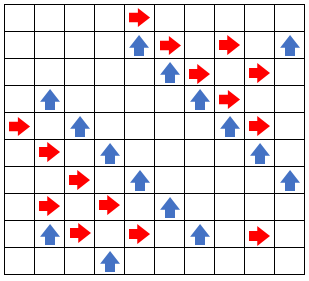
\includegraphics[width=0.4\textwidth]{ca1.PNG}\label{fig:ca1}}
  	\hfill
  	\subfloat[Jammed State]{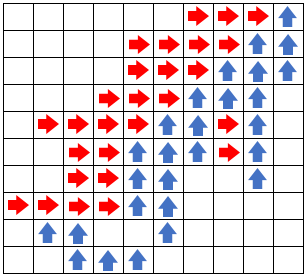
\includegraphics[width=0.4\textwidth]{ca2.PNG}\label{fig:ca2}}
  	\caption{Two states in the BML model. The red arrows are for eastward vehicles, while the blue arrows denote northward vehicles.}
\end{figure}


However, \shortciteA{M-BML:2016} modified the BML in such a way that it improved its performance. While the BML distributed the number of vehicles in eastwards and northwards equally, the M-BML distributed at random to be more realistic. In addition, current urban networks can be mapped immediately into the M-BML model for predicting traffic congestion.

% Knowledge-based
\shortciteA{Lee:KnowledgeBase}, meanwhile, developed a knowledge-based real-time travel time prediction model that uses location-based services (LBS) collected through data mining technologies. These LBS are collected from vehicles equipped with GPS and mobile data communication module to report its current speed, traveling direction and its current position. It also uses intersection delay patterns, discovered through sequential pattern mining, which is used to estimate the time to turn to an intersection. The model makes use of a dynamic linear combination of two weight predictors: the historical predictor and real-time predictor. Historical predictors are based on historical traffic information. It is used to estimate link travel time and predict intersection delays. On the other hand, the current predictor is based on real-time traffic information. It is used to incorporate external events into the travel time prediction of the model. The concept of dynamic linear combination allows the model to shift between these predictors. For instance, in the case of an external event (e.g. car accident), the model will reduce the weight of the historical predictor because the current predictor may be more reliable since the effect of this incident will immediately affect the traffic condition.

% H-ARIMA
The H-ARIMA model, on the other hand, makes use of 2 different submodels: ARIMA and HAM \shortcite{pan2012utilizing}. The ARIMA is an autoregressive moving average model that heavily relies on the combination of previous data collected just before the current time in determining the traffic condition for the next time series. Because it considers recent instances, the ARIMA is more optimal to use for short-term prediction. The HAM, on the other hand, relies more on the average of the previous data given that the data is on the same day of the week and at the same time of the day. In order to distinguish the most suitable approach for a given situation, The researchers trained a decision tree that selects which approach to use. Once given an input, the H-ARIMA feeds the input to both approaches and then gets the overall rate of the prediction error of both approaches. The overall rate of the prediction error is computed as the prediction error of the ARIMA divided by the sum of prediction errors of both approaches. If for instance, the rate of the ARIMA is less than the set threshold (0.5), it means that the ARIMA is to be used for the given situation.

% ANN AND SWT-ACNN
\shortciteA{Saputri2013} believed, however, that using ANN is the best method of forecasting amongst all others. Inspired by the nonlinear characteristics of Biological Brain System, the work performance of ANN can be compared to the workings of the human brain system. Besides its simple computation and fast performance, \shortciteA{ANN:2016} concluded that ANNs minimize the error in limited time; hence, it improves the efficiency and accuracy of the system. 

There were two models that used ANNs in their approach. One of them developed a traffic model that uses Jordan’s Sequential Neural Network, which has a good ability of generalization \shortcite{ANN:2016}. The structure of this kind of ANN is such that the distribution of nodes in the hidden layer should be the square of the number of nodes in the input layer. For example, if there are 5 nodes found in the input layer, then there must be 25 nodes in the hidden layer. The Jordan’s Neural Network contains four layers: (a) context layer, which acts as a memory and stores previous information, (b) input layer, which constitutes the input for the next processing, (c) hidden layer, which gets input from the “true” input layer and the context layer, and (d) output layer, which outputs the result or feedbacks to the context layer to be processed again. \figref{fig:annJordan} shows a Jordan’s Sequential Neural Network with 5 inputs in the input layer.

\begin{figure}[!t]
	\centering
	\captionsetup{justification=centering}
	\scalebox{.25}{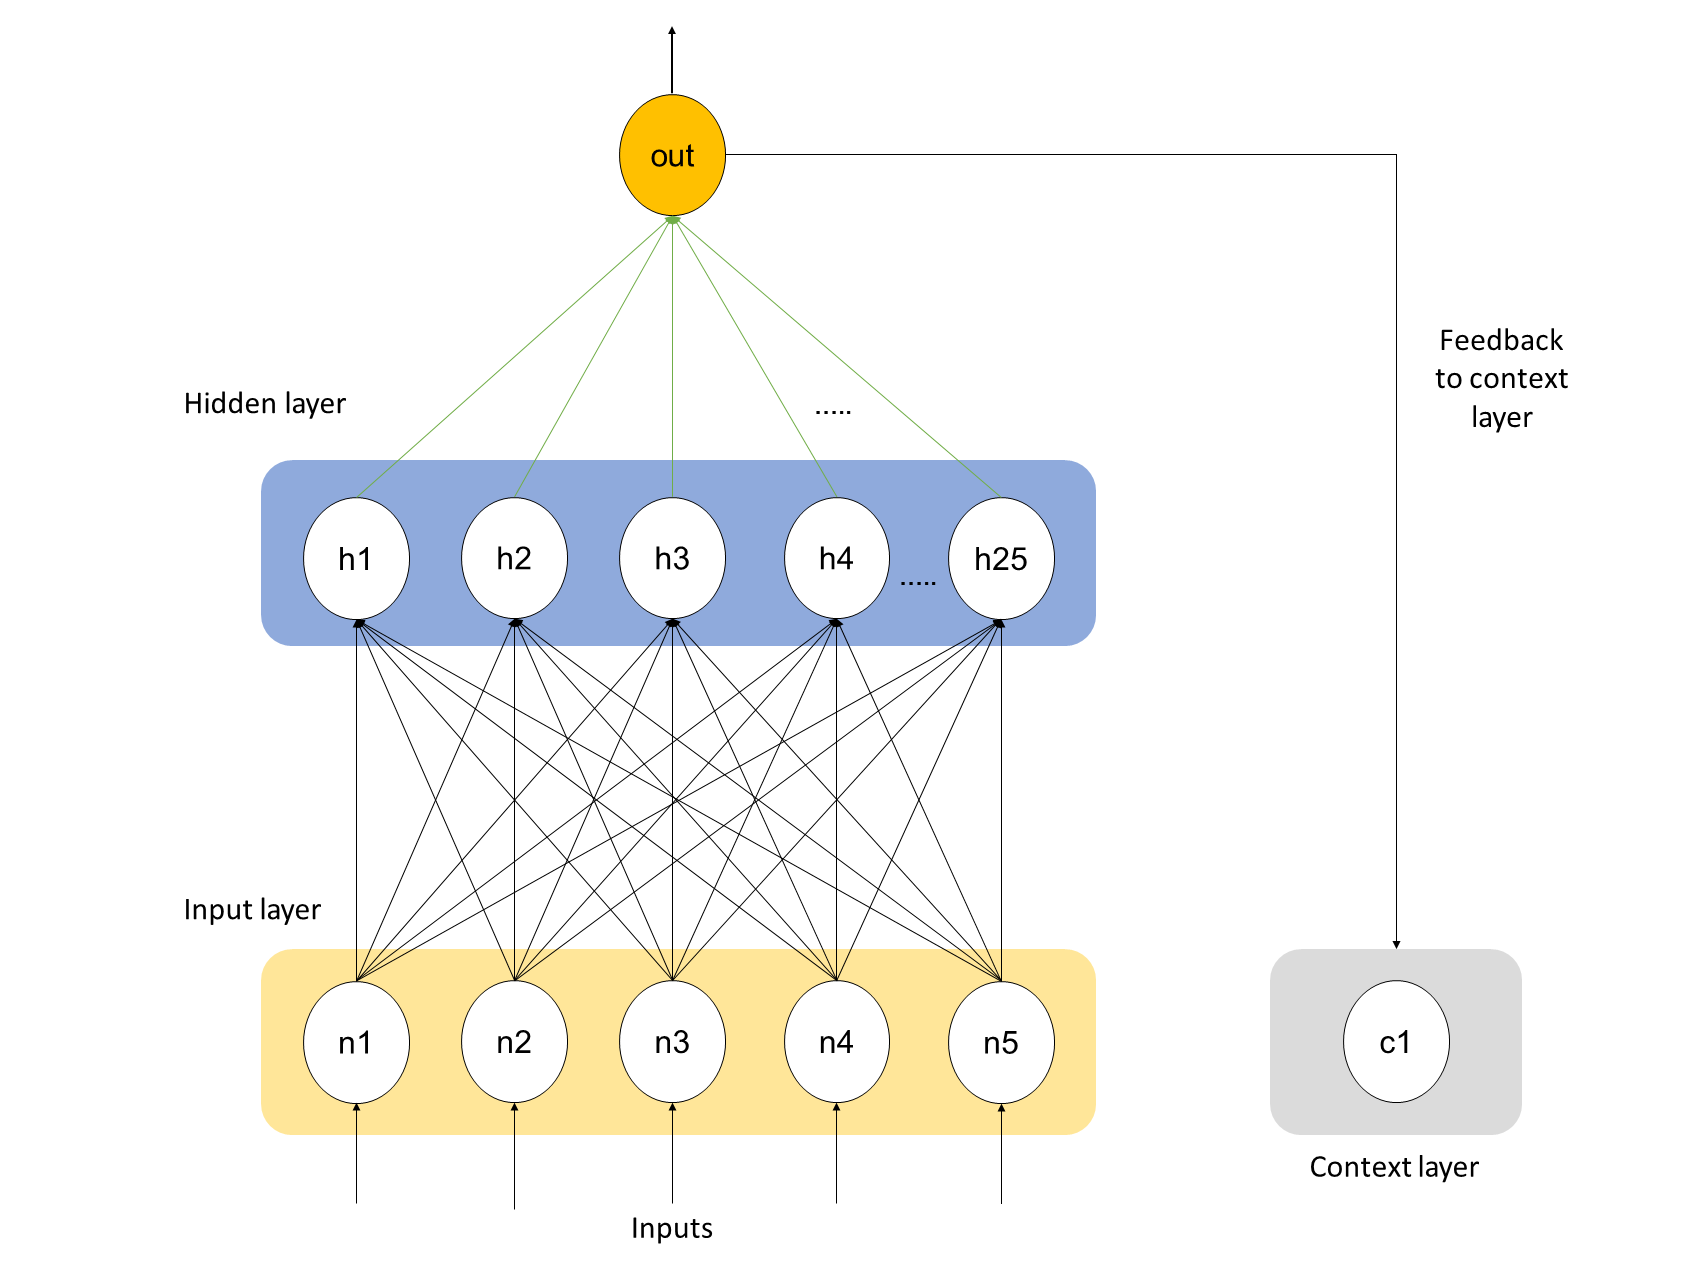
\includegraphics{ann.png}}
	\caption{ANN Framework used in More et al., 2016}
	\label{fig:annJordan}
\end{figure}

The ANN algorithm in the SWT + ACNN model, on the other hand, uses the structure of FeedForward (FF) Back Propagation (BP) algorithm for training \shortcite{dunne:2013}. The FF phase receives the input and passes it to the output layer through the hidden layer. As discussed earlier, the input fed into the neural network of the SWT + ACNN model is generated from auto-correlation. The output values are calculated from the input layer passing through the hidden layer, and is summed with the weights of the neural network units through activation functions. The BP phase compares the generated to the desired value. This phase optimizes the error function through a number of iterations until the error function is close to optimal. The ANN used by the SWT + ACNN, which takes in auto-correlated inputs, have been labeled as the Auto-Correlation Neural Network (ACNN).

% DBN with Data Fusion
In the developed model of \shortciteA{koesdwiady:2016}, Deep Belief Network (DBN) and data fusion techniques are used to enhance the generated prediction. DBN, unlike ANN, is composed of multiple layers of hidden units. The DBN of this model makes use of Restricted Boltzmann Machines (RBM), and stacks RBM together within the hidden layer. RBM is an unsupervised learning algorithm that can learn useful features of the data. It takes the input and translates them into a set of numbers that represents them. Then, these numbers can be translated back to reconstruct the inputs. This neural network is trained through multi-task learning to predict several traffic flow predictions at each level at the same time to reach the final traffic flow prediction. \shortciteA{koesdwiady:2016} further discusses that the optimal architecture for the DBN in traffic prediction consists of three hidden layers with 250 in the first, 200 in the second, and 100 in the last hidden layer. Additionally, \shortciteA{koesdwiady:2016} adds that 100 epochs is optimal for training the DBN. The separately predicted traffic flow and weather data will be fused using data fusion techniques to generate an enhanced and accurate traffic flow prediction. The DBN with Data Fusion makes use of Decision In - Decision Out (DEI-DEO) which fuses input data considered as the decision to generate a new or enhanced decision \shortcite{koesdwiady:2016}.

% RNN using LSTM
\shortciteA{Jia:2017} used RNN using LSTM to capture time series characteristics during its training and prediction phases. RNN uses memory cells to save information from previous time intervals. LSTM can adjust its hyperparameters to automatically adjust its hyperparameters from the data. The LSTM model consist of one input layer, one hidden layer, and one output layer. The hidden layer performs as the network's memory block that memorizes the long and short term temporal features. 

% MLRA
\shortciteA{Lee2015}, on the contrary, suggested a traffic model that makes use of multiple linear regression analysis (MLRA) employing both weather forecast data and traffic congestion data. MLR analysis is used to explain the relationship between one continuous dependent variable (traffic congestion data) and two or more independent variables (weather data). In this model, the traffic congestion is influenced by 48 independent variables. However, in their research, some of those independent variables are highly correlated to each other, and therefore should be removed to prevent the increase of correlation. 






\section{Evaluation Strategy}
Before computing the accuracy of each traffic models, different experiments and case studies were first performed. All traffic models were tested to predict the traffic congestion at a given time period.

% knowledge-based
In evaluating the knowledge-based model, \shortcite{Lee:KnowledgeBase} collected five months of location-based service (LBS) raw data. The LBS raw data was collected through an online taxi dispatch system (TDS), consisting of around 500 taxis operating 24-7 in a Taipei urban area. The first four months are used for mining traffic patterns, whereas the fifth is used for verifying the accuracy of the model. In the experiment, a random origin-destination pair is selected at two peak hour sections. The model produced a precision of 10.8\% \textit{relative mean error} (RME) and \textit{root mean squared error} RMSE of 15.92\%. To further challenge its reliability, the experiment was performed with the same set of input, having the intersection delay replaced with a turning delay estimate from a human expert. The model produced a precision of 20\% RME and 30.55\% RMSE, which, in comparison with the pattern generated intersection delay, is relatively unreliable. 

% H-ARIMA
In evaluating the accuracy of the H-ARIMA model, the researchers compared results with other baseline approaches given two situations: short-term prediction and long-term prediction \shortcite{pan2012utilizing}. RMSE and \textit{mean absolute percentage error} (MAPE) were used to measure the accuracy of the traffic prediction. Although the H-ARIMA model was able to yield better results than the other baseline approaches for short-term prediction, the researchers were not able to see the edge of the H-ARIMA model against them. Similar to that, the H-ARIMA model was also able to produce a better result for long-term prediction compared to the baseline approaches. It was observed that its MAPE is lower compared to others because it considers historical traffic data in predicting traffic. Overall, the H-ARIMA model was able to produce around 95-96\% accuracy.

% DBN with Data Fusion
To measure the accuracy of the predictions of the DBN with Data Fusion, performance indexes RMSE and MAE are used \shortcite{koesdwiady:2016}. These performance indices calculate the error value of the prediction by comparing the actual and predicted output at a certain time \textit{t}. The research compared the performance of different neural networks of ARIMA and ANN with DBN. After experimentation, the DBN outperformed the other neural networks in predicting traffic flow. The performance of the DBN generated an average MAE of 0.07 and average RMSE of 0.05. On the other hand, ANN generated an average MAE of 0.08, and an average of RMSE of 0.06, and ARIMA generated an average MAE of 0.27 and an average RMSE of 0.23.

To examine the performance of the neural network with low, medium and heavy traffic, three different freeways that experience the mentioned traffic conditions are chosen \shortcite{koesdwiady:2016}. The detrended version of the data was more accurate in predicting heavy traffic, and the original data was more accurate in predicting low and medium traffic. Medium traffic flow using original data achieved an MAE of 0.041 and RMSE of 0.06. Low traffic flow using original data achieved MAE of 0.034 and RMSE of 0.045.On the other hand, detrended version of the data performed best in predicting high traffic flow achieving an MAE of 0.06 and RMSE of 0.09. Moreover, using weekday/weekend version of the data generated a higher average error. Furthermore, the model better predicts the medium traffic flow with consideration to weather information.

For \shortciteA{Jia:2017}, they evaluated the model, and its effectiveness in predicting traffic with consideration of rainfall, through comparing the performances of DBN and LSTM models with and without rainfall consideration. The test dataset used for evaluating consist of instances when rainfall was significantly present. The study used MAE, MAPE and RMSE as the evaluation metrics. Results show that predicting 10-minute traffic volume is more accurate than predicting a 30-minute traffic volume. Moreover, the LSTM model performed better than DBN with or without considering rainfall, showing the advantage of LSTM to capture time series patterns of the traffic data. The LSTM model achieved an RMSE (vel/h) of 240.98 and  269.91 for the 10-minute and 30-minute prediction, respectively, while the DBN model achieved an RMSE (vel/h) of 255.79 and 365.49, showing a significant change from the performance of LSTM. 

% SWT-ACNN
The model’s performance was compared to ANN that takes in undecomposed data to observe the differences in performance. To measure the accuracy and performance, RMSE and MAPE were used. The SWT-ACNN outperformed the non-wavelet model significantly by approximately 5\% of MAPE, and 40 of RMSE. Additionally, the wet model is superior to the dry model achieving a MAPE of more than 30\% than the dry model.

To compare the results of \shortciteA{Lee2015}’s MLRA model with the actual values, present traffic congestion data were used. As discussed in the previous section, the weather data used in their research are temperature, humidity, rainfall. In their analysis, they used MAPE to assess the developed MLRA model. When they predicted the traffic congestion from July and August 2013, the traffic model got an accuracy of 94.1\%. However, when they predicted the traffic congestion in 2014 for the same months, they have arrived at 84.8\%. %This may be because the weather and traffic congestion data used to create this model came from July and August 2013.




\begin{sidewaystable}
	\caption{Summary of Traffic Models}
    \centering
    \begin{tabular}{| L{3cm} | L{3cm} | L{3cm} | L{3cm} | L{3cm} | L{3cm} | L{2cm} |} 
    
    \hline
    Author (Year) & Modeling Approach & Traffic Data Input & Weather Data Input & Coverage & Evaluation Strategy & Accuracy \\
    
    \hline
    \shortciteA{M-BML:2016} &
    Cellular Automata (CA)  &
    - traffic density \newline - evolution rules &  
    none & 
    - road segment \newline - Birmingham, England & 
    not indicated &
    94.00\% \\
    
    \hline
    \shortciteA{ANN:2016} &
    Artificial Neural Network (ANN) &
    traffic volume &
    none &
    - road segment \newline - Dublin, Ireland & 
    not indicated &
    92.00 - 98.00\% \\
    
    \hline
    \shortciteA{Lee:KnowledgeBase} &
    Knowledge-based &
    - vehicle GPS data
    \newline
	- intersection delay & 
    none &
    - whole city
    \newline
	- Taipei, Taiwan &
    - RMSE
    \newline
    - RME
    &
    84.08\% \\

	\hline
    \shortcite{pan2012utilizing} & 
    HAM and ARIMA (H-ARIMA) &
    - traffic volume
    \newline
	- speed &
    none &
    - road segment
    \newline
	- Los Angeles, USA &
    - RMSE
    \newline
    - MAPE
    &
    95.99\% \\

	\hline
    \shortciteA{koesdwiady:2016} &
    Deep Belief Network with Data Fusion (DBN with Data Fusion) &
    - traffic volume &
    - temperature
    \newline
    - wind gust
    \newline
    - weather condition &
    - road segment
    \newline
    - San Francisco, USA &
    - RMSE
    \newline
    - MAE
    &
    95.95\% \\
    
    \hline
    \shortciteA{dunne:2013} &
    Stationary Wavelet Transform and Auto-Correlation Neural Networks (SWT-ACNN) &
    - traffic volume &
    - rainfall &
    - road segment
    \newline
    - Dublin, Ireland & 
    - RMSE
    \newline
    - MAPE
    &
    91.45\% \\
    
    \hline
    \shortciteA{Lee2015} &
    Multiple Linear Regression Analysis (MLRA) &
    - speed 
    \newline
    - travel time
    \newline
    - traffic volume &
    - temperature &
    - whole city 
    \newline
    Seoul, South Korea &
    - MAPE &
    84.80\% \\
    
    \hline
    
    \end{tabular}
\end{sidewaystable}
